% !TEX root = ../0_tcc.tex

\begin{figure}[H]
	\centering
	\begin{subfigure}{\textwidth}
		\centering
		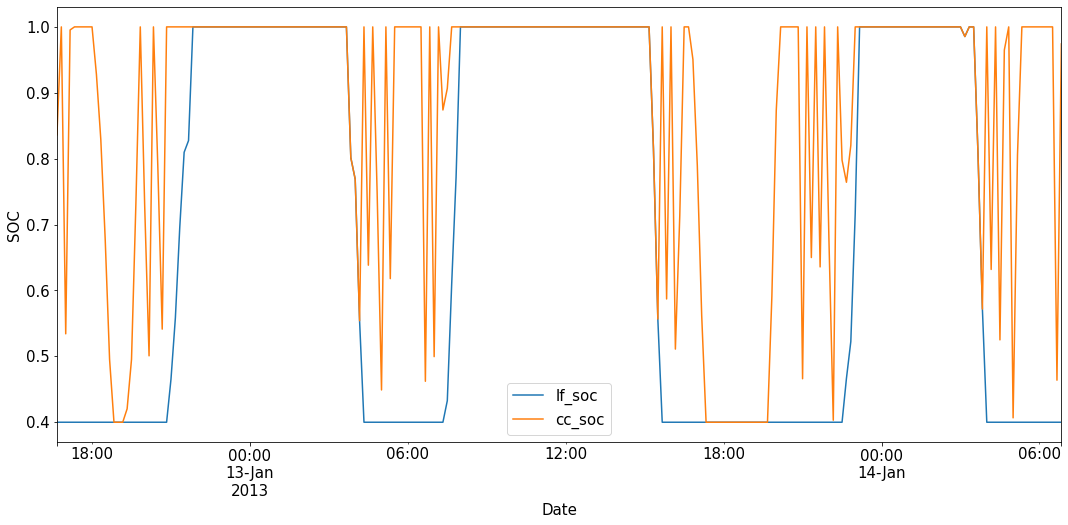
\includegraphics[width=0.7\textwidth]{../img/soc.png}
		\caption{Sem tempo mínimo de funcionamento}\label{fig:soc0}
	\end{subfigure}
	\\ \vspace{1cm}
	\begin{subfigure}{\textwidth}
		\centering
		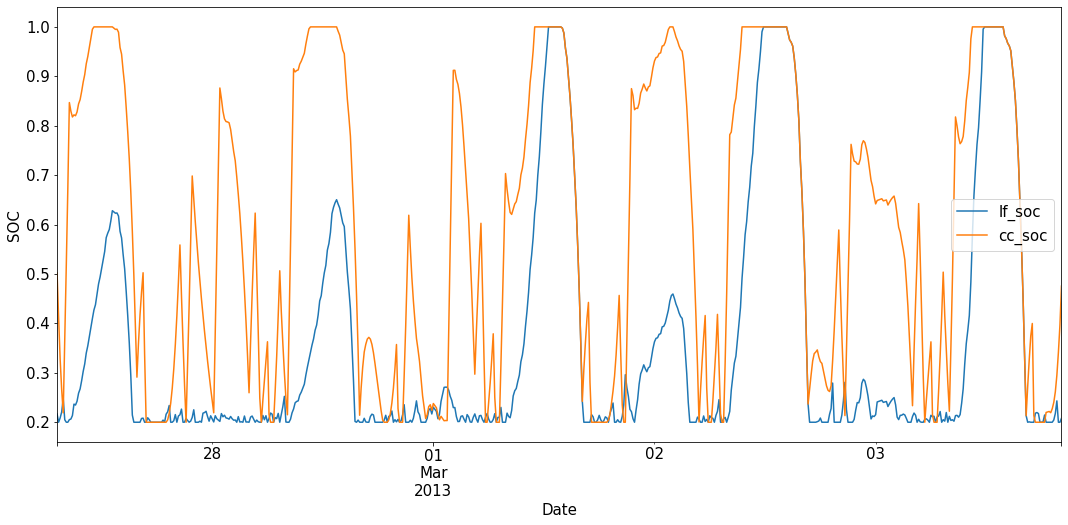
\includegraphics[width=0.7\textwidth]{../img/soc_3.png}
		\caption{Mínima excecução de 3 intervalos}\label{fig:soc3}
	\end{subfigure}
	\\ \vspace{1cm}
	\begin{subfigure}{\textwidth}
		\centering
		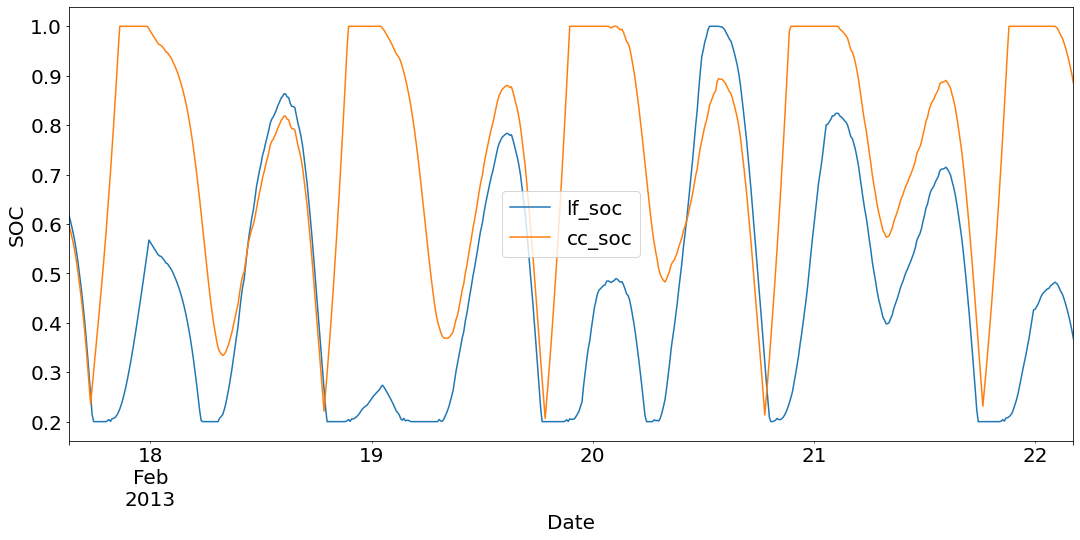
\includegraphics[width=0.7\textwidth]{../img/soc_6.png}
		\caption{Mínima excecução de 6 intervalos}\label{fig:soc6}
	\end{subfigure}
	\caption{Comparação da oscilação do \acrshort{soc}}\label{fig:soc}
\end{figure}
